
  
\label{sec:evaluation}

 

%\section{Preliminary Evaluation}
%\label{sec:eval}
%
%\begin{figure*}[!htp]
%  \begin{minipage}{0.16\textwidth}
%\begin{center}
%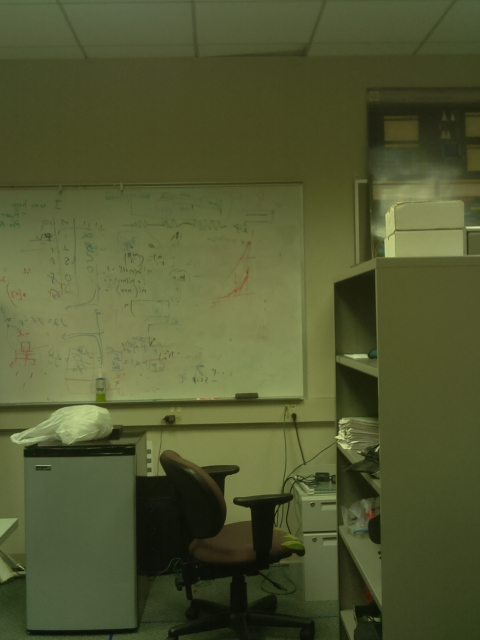
\epsfig{file=figs/pic0.jpg,height=1in,width=1in}
% \end{center}
%\end{minipage}
%\begin{minipage}{0.16\textwidth}
%\begin{center}
%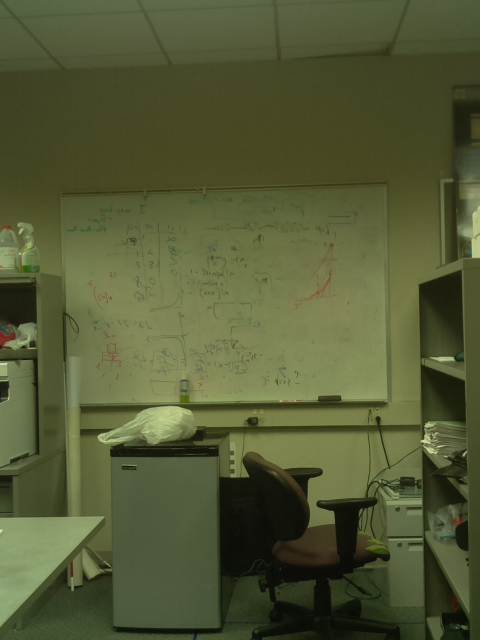
\epsfig{file=figs/pic1.jpg,height=1in,width=1in}
% \end{center}
%\end{minipage}
%\begin{minipage}{0.16\textwidth}
%\begin{center}
%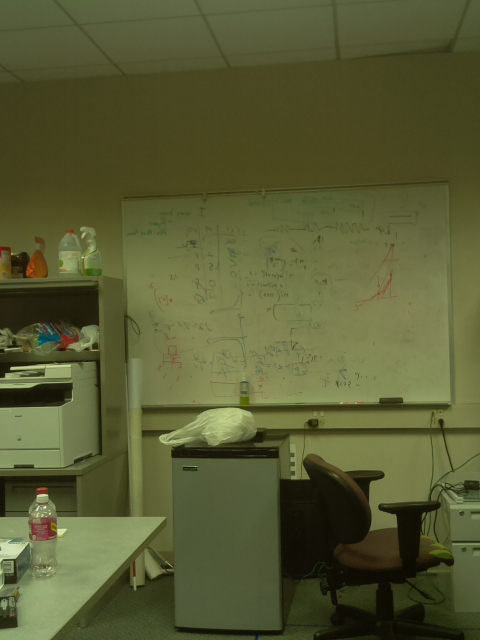
\epsfig{file=figs/pic2.jpg,height=1in,width=1in}
% \end{center}
%\end{minipage}
%\begin{minipage}{0.16\textwidth}
%\begin{center}
%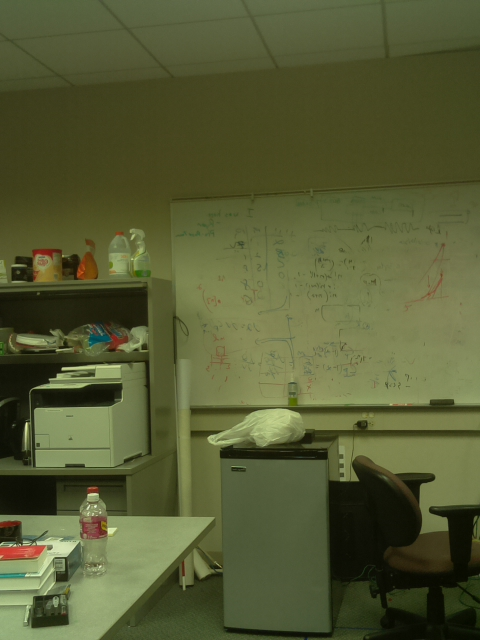
\epsfig{file=figs/pic3.jpg,height=1in,width=1in}
% \end{center}
%\end{minipage}
%\begin{minipage}{0.16\textwidth}
%\begin{center}
%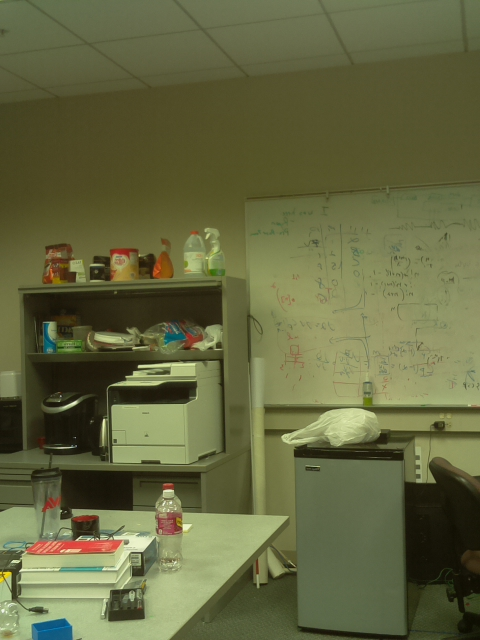
\epsfig{file=figs/pic4.jpg,height=1in,width=1in}
% \end{center}
%\end{minipage}
%\begin{minipage}{0.16\textwidth}
%\begin{center}
%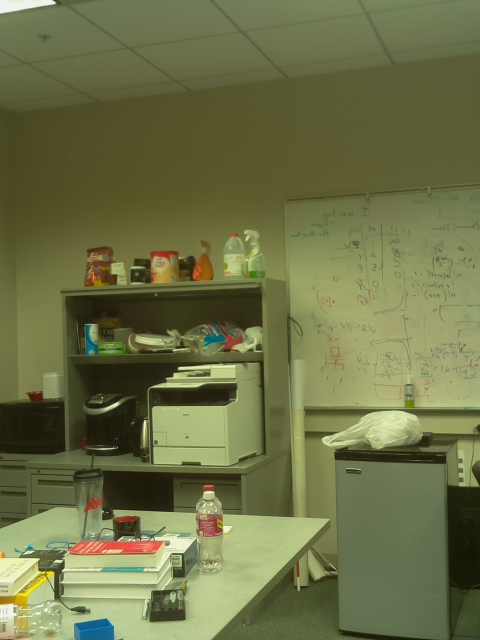
\epsfig{file=figs/pic5.jpg,height=1in,width=1in}
% \end{center}
%\end{minipage}
%\begin{minipage}{0.16\textwidth}
%\begin{center}
%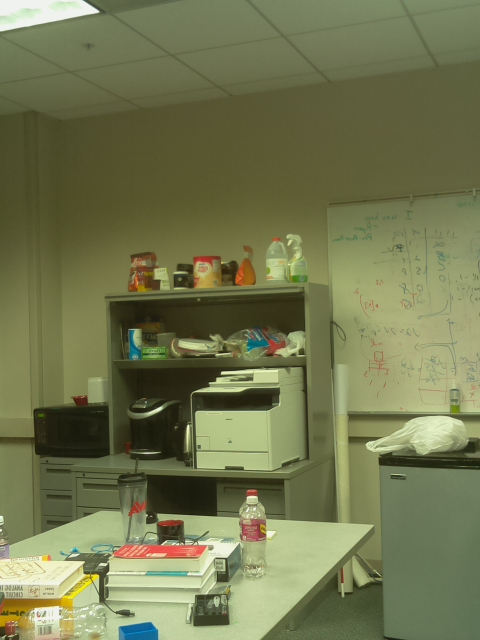
\epsfig{file=figs/pic6.jpg,height=1in,width=1in}
% \end{center}
%\end{minipage}
%\begin{minipage}{0.16\textwidth}
%\begin{center}
%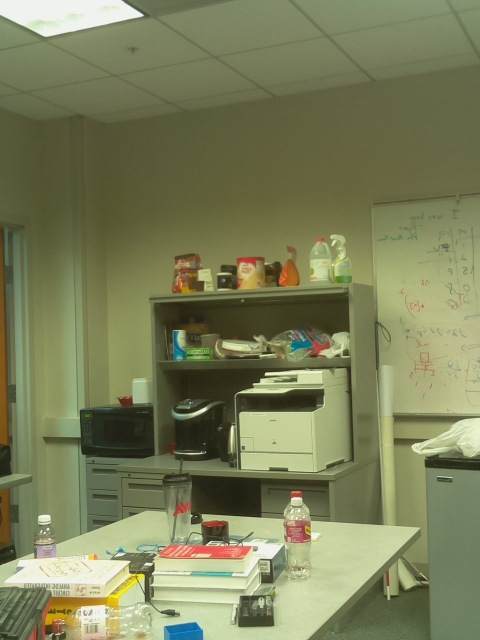
\epsfig{file=figs/pic7.jpg,height=1in,width=1in}
% \end{center}
%\end{minipage}
%\begin{minipage}{0.16\textwidth}
%\begin{center}
%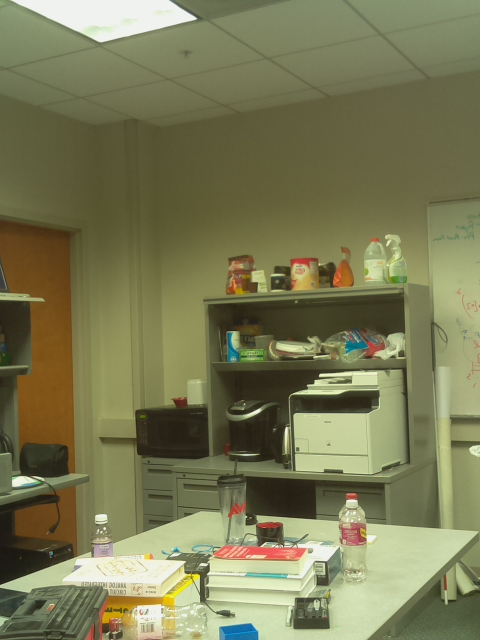
\epsfig{file=figs/pic8.jpg,height=1in,width=1in}
% \end{center}
%\end{minipage}
%\begin{minipage}{0.16\textwidth}
%\begin{center}
%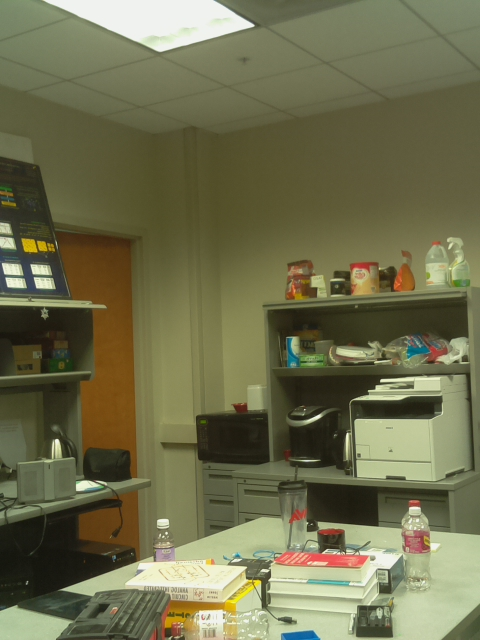
\epsfig{file=figs/pic9.jpg,height=1in,width=1in}
% \end{center}
%\end{minipage}
%\begin{minipage}{0.16\textwidth}
%\begin{center}
%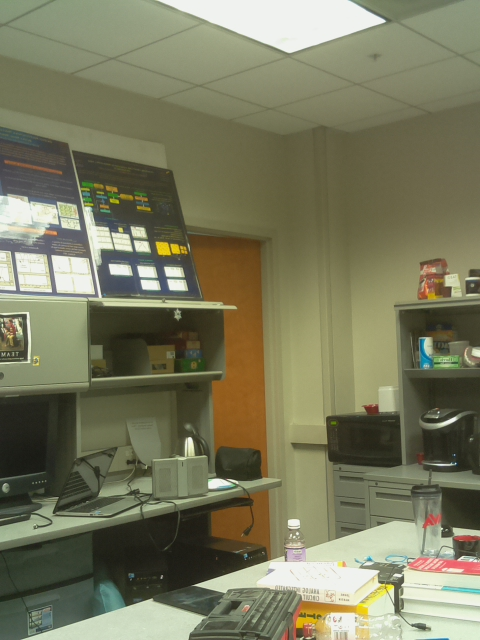
\epsfig{file=figs/pic11.jpg,height=1in,width=1in}
% \end{center}
%\end{minipage}
%\begin{minipage}{0.16\textwidth}
%\begin{center}
%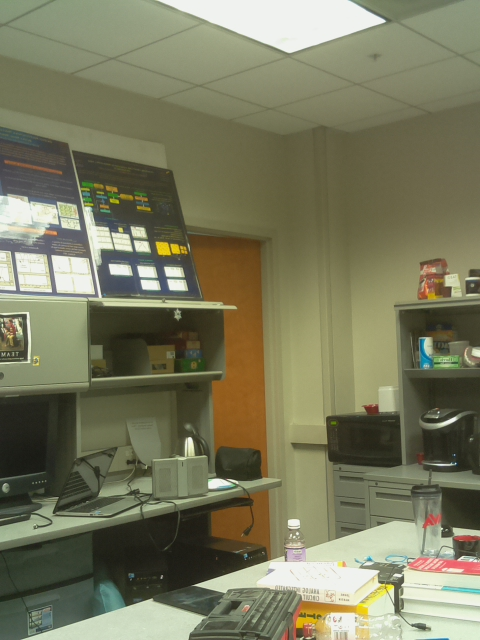
\epsfig{file=figs/pic11.jpg,height=1in,width=1in}
% \end{center}
%\end{minipage}
%\caption{Baseline Stream of Images}
%\label{fig:Individual}
%\end{figure*}
%
%
%
%\begin{figure}[!hpt]
%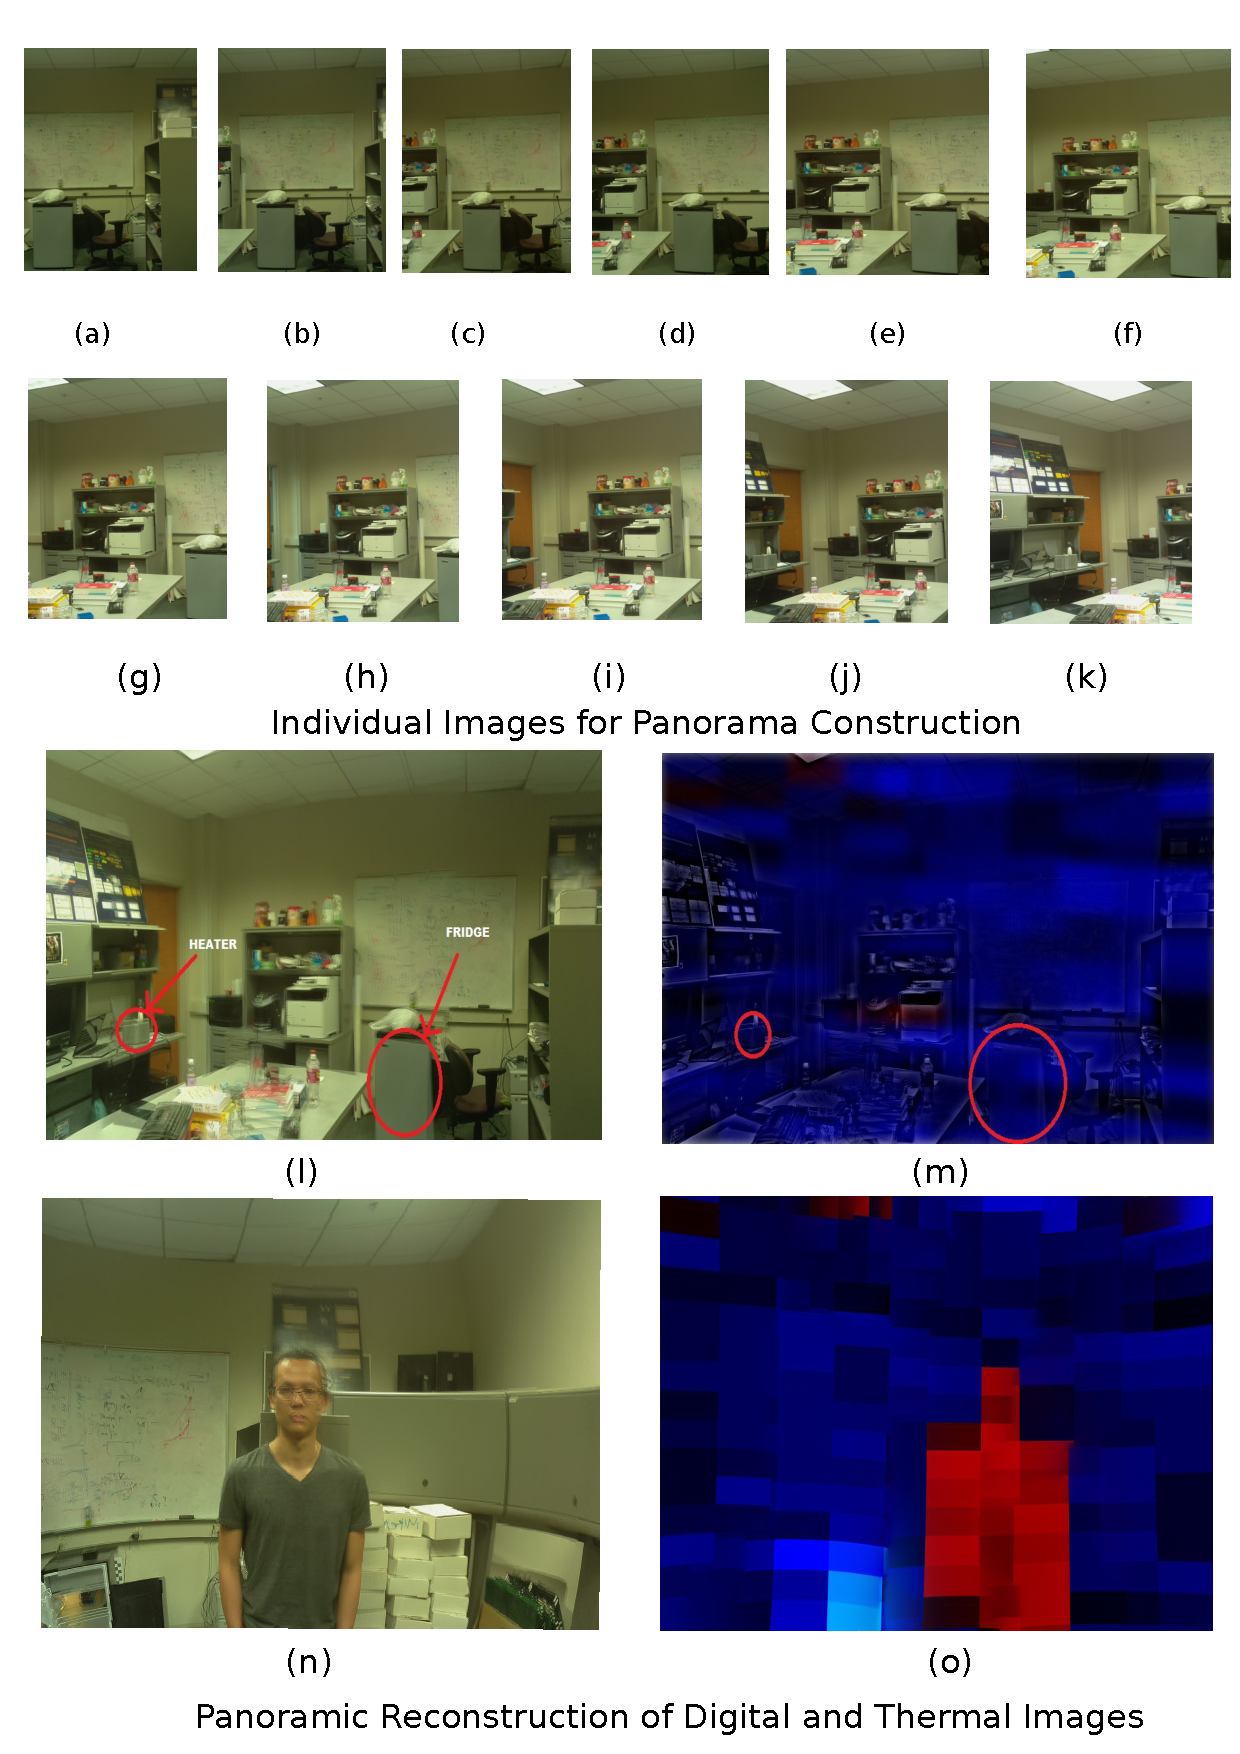
\epsfig{file=figs/panorama,height=3.5in,width=3.2in }
%\caption{Digital and Thermal Image Stitching Results}
%\label{fig:Stitch}
%\end{figure}


%\begin{figure}[!hpt]
%	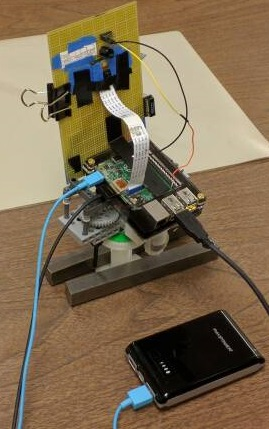
\epsfig{file=figs/SystemDiagram,height=1in,width=1.2in }
%	\caption{Digital and Thermal Image Stitching Results}
%	\label{fig:Stitch}
%\end{figure}
%
%\begin{figure}[!htp]
%\begin{minipage}{0.00\textwidth}
%\mbox{}
%\end{minipage}
%\begin{minipage}{0.48\textwidth}
%\begin{center}
%\scriptsize{
%\fbox{\parbox{5cm}{\texttt{
%\begin{tabbing}
%\=Procedure IPU(Input: Individual set of baseline digital \\
%\;\; images($D$) and corresponding thermal images ($I$)) \\
%\> Output: Thermal Panoramic Image\\
%1. \= Create panoramic image for the\\ 
%\;\;baseline digital images using Hugin tool\\
%2. \> Replace the digital images with the thermal images\\ 
%\;\; and load the saved project again to construct the\\ 
%\;\;panoramic thermal image\\
%3. \> Employ High pass filter on the digital image \\
%4. \> Employ Low pass filter on the IR image \\
%5. \> Combine the two to get masked thermal image
%\end{tabbing}}}}}
%\caption{IPU procedure}
%\label{algo:IPU}
%  \end{center}
%  \end{minipage} 
%\end{figure}


 \section{Evaluation}

    \indent In this section we discuss the analytics using the panoramic thermal images. We perform initial set of experiments which includes discerning among cold surfaces, hot surfaces and human bodies. The purpose is to identify - \textit{ Appliance States/Energy Wasting Appliances} and also \textit{ Occupancy Detection}. In Table~\ref{table:temp} the list of objects, their temperature for appliances and objects which has effect of energy consumption. We collected data from two locations - LAB 1 and LAB 2. LAB 1 is much colder inside and have an average temperature of 71-73$^{\circ}$F and the LAB 2 is an older building with poor ventilation and have windows which can be opened. The average temperature there is 78-81$^{\circ}$F. The appliances present in the different labs are listed in Table~\ref{table:temp}. For ground truth validation we used a commercial Infrared thermometer and took multiple readings to get the range of temperature values.
   

\begin{table}[h!]
\centering
 \begin{tabular}{||p{1.3cm} | p{2cm} | p{2cm} | p{1cm}||}
 \hline
 Object & Temperature Appliance OFF(F) & Temperature Appliance ON(F) & Setting Location\\ [0.5ex]
 \hline\hline
 Wall  & - & 73 & LAB1\\
  \hline\hline
 Wall  & - & 77-81 & LAB2\\
  \hline
 Fridge & 73 & 50 & LAB1 \\
 \hline
 Fridge & 75  & 50-55 & LAB2 \\
 \hline 
 Freezer & 75  & 50-55 & LAB2 \\
 \hline
 Heater & 74 & 120 &  LAB1\\ 
 \hline
  Heater & 74 & 100-140 &  LAB2\\ 
 \hline
 Coffee-Maker & 72-77 & 90-180 &  LAB2\\
 \hline
 Microwave & 77-78 & 77-78 & LAB2\\
 \hline
 Window & 76-77 & 75 & LAB2\\ [1ex]
 \hline
 \end{tabular}
 \label{table:temp}
\caption{Temperature of different Surfaces}
\end{table}


 \indent There are three possible types of thermal regions in an image - background, cold region and hot region. The image that needs to be segmented is the stitched IR image and the objective is to create a thermal mask which separates the hot and cold regions from the background. Since the thermal image is being used for segmentation, the results are subjected to the choice of color palette and range selection.  We ensure that the background has darker tones than the hot or cold surfaces which helps achieve the desired segmentation after image binarization using Otsu's method~\cite{Otsu}. We apply a 7$\times$7 neighborhood 2-D median filter to eliminate small blobs and get the few major thermal zones. Next step is to find the contour and their location of the blobs and then for each blob the average temperature is computed and the lookup table~\ref{table:temp} is used to identify the object closest to that temperature. A pseudocode for the entire procedure has been given in~\ref{algo:Two Object}.
 
 
 \begin{figure}[!htp]
\begin{minipage}{0.00\textwidth}
\mbox{}
\end{minipage}
\begin{minipage}{0.48\textwidth}
\begin{center}
\scriptsize{
\fbox{\parbox{5cm}{\texttt{
\begin{tabbing}
\=Procedure Hot and Cold Zone Segmentation(Input: \\Constructed panoramic thermal image ($I$)\\
\> Output: Matched Thermal Regions\\
1. \= Apply Otsu's thresholding\\
2. \> Find the contours of the hot and cold regions\\
3. \> Match the internal temperatures with the \\LIST OF SURFACE TEMPERATURES\\
\end{tabbing}}}}}
\caption{Thermal region identification: Two object case Hot and Cold}
\label{algo:Two Object}
  \end{center}
  \end{minipage}
\end{figure}

    \subsection{Appliance State Detection/Energy Wasting Object Detection:} In this section we discuss the experiments performed using the mentioned methods for Appliance State Detect or Energy Wasting Object Detection. By an appliance state we mean an appliance turning 'ON' and those who generate heat when turned ON. For example Coffee-Maker and Heater both generate heat when turned ON. In Fig~\ref{fig:Object Detection}, it is shown that the Heater and Coffee-Maker and be distinctly distinguished as two hot sources when they are kept at a distance of about 2 feet apart. However the temperature value for both the appliances can vary in a range and distinguishing them using the particular lookup becomes difficult. \\
   \indent Discerning two definite thermal regions become difficult when they are in close proximity. For example in case of the Fridge-Freezer Fig~\ref{fig:Object Detection}, the location is determined as cold zone as a whole and not separately as Fridge and Freezer. The open window in Lab 2 can't be detected as the difference between inside and outside temperature was less. In Lab 1, we took data for two humans and an open fridge and a heater turned 'ON' and all the objects could be detected Fig~\ref{fig:Object Detection}.
   
 \begin{figure}[!ht]
 	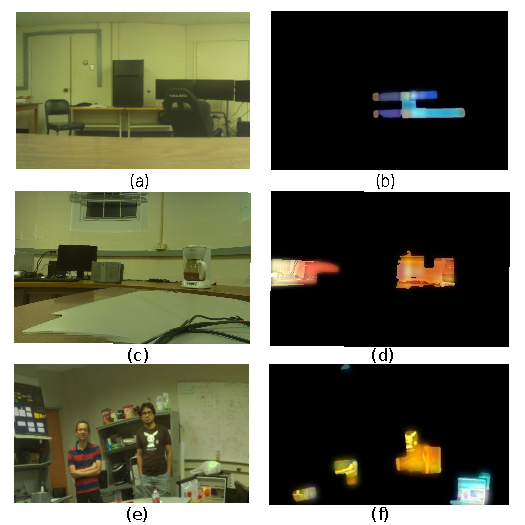
\epsfig{file=figs/Appliance.pdf,height=3in,width=3.2in} 
 	\label{fig:Object Detection}
 	\caption{Appliance and Object Detection Results}
 \end{figure}
    
    \begin{table}[h!]
    	\centering
    	\begin{tabular}{||p{1.8cm} | p{1.2cm} | p{1.2cm}| p{1cm} | p{1cm}||}
    		\hline
    		Event & Detected & Est. Temp. & Actual Temp & Location\\ [0.5ex]
    		\hline\hline
    			Heater ON  & Yes & 108 &  120 & LAB1\\
    			\hline
    			 Fridge Open  & Yes & 98 &  100 & LAB1\\
    			 \hline
    			 Man 1 Standing  & Yes & 99 &  81 & LAB1\\
    			\hline
    				 Man 2 Standing  & Yes & 103 &  83  & LAB1\\
    				 \hline
    		 Heater ON  & Yes & 110 &  120 & LAB2\\
    		\hline
		     Coffee ON  & Yes & 98 &  100 & LAB2\\
    		\hline
    		 Fridge Open  & Yes & 98 &  100 & LAB2\\
    		\hline
    		Fridge \& Freezer Open  & No & 98 &  100 & LAB2\\
    		\hline
    		Man Hoodie  & No & 80 &  78 & LAB2\\
    		\hline
    		Man No-Hoodie & No & 80 &  78 & LAB2\\
    		\hline
    		Window Open & No & 78 &  75 & LAB2\\
    		\hline\hline
     	\end{tabular}
    	\label{table:DetectionTable}
    	\caption{Results Table}
    \end{table}
    
    
     \subsection{Occupancy Detection} In this section we discuss the experiments performed for occupancy detection. Body heat can be detected through thermal imaging. In case of the Fig~\ref{fig:Occupancy} it can be seen that two distinct human beings can be detected. However, for this technique to work the body temperature has to be significantly more than the background temperature. We don't consider a case where the room is much hotter than body temperature as that is an improbable scenario. The temperature measured by the IR is the radiation from the human body. However this is subjected to variation - for example we considered two cases where a human is wearing a hoodie and not wearing one in Fig~\ref{fig:Occupancy}. It was found that the one wearing hoodie has lower temperature than the one not wearing hoodie. This creates a problem when the room temperature becomes same as that of the human body and detection of bodies is difficult. We found that its easier to identify a person in LAB 1 which has colder temperature than the one at LAB 2, as LAB2 had poor air-conditioning and hence hot. 


 \begin{figure}[!h]
 	\begin{center}
 		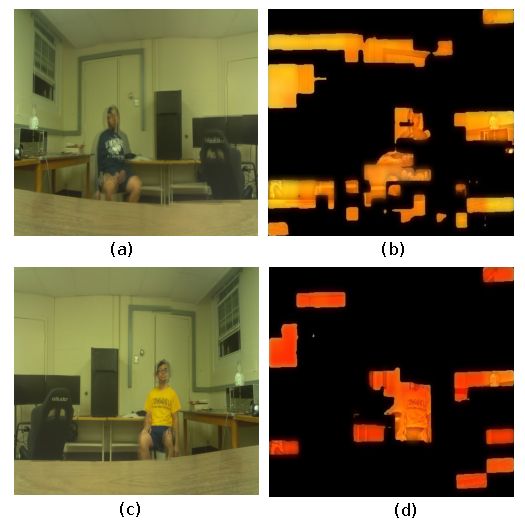
\epsfig{file=figs/Occupancy.pdf,height=2.in,width=2.5in}
 	\end{center}
 	\caption{Occupancy Detection Results}
 	\label{fig:Occupancy}
 \end{figure}




 